% ============================================================
% SACHIEL — A JUPITER IN CANCER CEREMONY
% ============================================================
% Compiled with XeLaTeX
% Booklet format: 8.5x11 printed duplex, folded to 5.5x8.5
% Font: TeX Gyre Pagella (Palatino clone)
% ============================================================

\documentclass[10pt,openany]{book}

% --- Document metadata ---
\newcommand{\docversion}{1.2}

% --- Typographic constants ---
\newcommand{\prayersize}{\Large}
\newcommand{\rubricsize}{\large}
\newcommand{\attributionsize}{\footnotesize}

% --- Page geometry ---
\usepackage[
  paperwidth=5.5in,
  paperheight=8.5in,
  top=0.55in,
  bottom=0.55in,
  inner=0.55in,
  outer=0.55in,
  includehead
]{geometry}

% --- Font setup ---
\usepackage{fontspec}
\setmainfont{texgyrepagella-regular.otf}[
  Ligatures=TeX,
  Numbers=OldStyle,
  BoldFont=texgyrepagella-bold.otf,
  ItalicFont=texgyrepagella-italic.otf,
  BoldItalicFont=texgyrepagella-bolditalic.otf
]

% --- Essential packages ---
\usepackage{graphicx}
\usepackage{microtype}
\usepackage{xcolor}
\usepackage{titlesec}
\usepackage{fancyhdr}
\setlength{\headheight}{20pt}

% --- Colors ---
\definecolor{rubricsred}{RGB}{160, 40, 40}
\definecolor{deepgold}{RGB}{120, 90, 20}
\definecolor{darkgrey}{RGB}{60, 60, 60}
\definecolor{lightgrey}{RGB}{200, 200, 200}
\definecolor{jupiterblue}{RGB}{40, 60, 120}

% --- Rubric command ---
\newcommand{\rubric}[1]{%
  {\rubricsize\itshape\color{rubricsred} #1}%
}

% --- Section title formatting ---
\titleformat{\chapter}[display]
  {\normalfont\large\bfseries\centering\color{deepgold}}
  {}
  {0pt}
  {\rule{\linewidth}{0.4pt}\\[4pt]\MakeUppercase}
  [\vspace{2pt}\rule{\linewidth}{0.4pt}]

\titleformat{\section}
  {\normalfont\normalsize\bfseries\centering\color{darkgrey}}
  {}
  {0pt}
  {\MakeUppercase}

\titleformat{\subsection}
  {\normalfont\small\itshape\centering\color{rubricsred}}
  {}
  {0pt}
  {}

% --- Spacing ---
\titlespacing*{\chapter}{0pt}{-5pt}{12pt}
\titlespacing*{\section}{0pt}{10pt}{4pt}
\titlespacing*{\subsection}{0pt}{6pt}{2pt}

% --- Header/footer ---
\pagestyle{fancy}
\fancyhf{}
\fancyhead[LE]{\small\itshape\color{darkgrey} Sachiel}
\fancyhead[RO]{\small\itshape\color{darkgrey} Full Moon in Sagittarius}
\fancyfoot[C]{\small\color{darkgrey}\thepage}
\renewcommand{\headrulewidth}{0.2pt}
\renewcommand{\headrule}{\hbox to\headwidth{\color{lightgrey}\leaders\hrule height \headrulewidth\hfill}}

% --- Liturgical mark font ---
\newfontfamily\liturgicalfont{Symbola}

% --- Planetary/astrological symbol (Symbola inline) ---
\newcommand{\ps}[1]{{\liturgicalfont #1}}

% --- Versicle/response ---
\newcommand{\versicle}[1]{{\color{rubricsred}\liturgicalfont ℣}~#1}
\newcommand{\response}[1]{{\color{rubricsred}\liturgicalfont ℟}~#1}

% --- Prayer block ---
% \linespread before \prayersize so the \selectfont inside \Large picks it up;
% corrects OTF ascent/descent metrics overrunning the default 17pt baselineskip.
\newcommand{\prayerblock}[1]{%
  {\linespread{1.2}\prayersize\noindent #1\par}%
}

% --- Ornamental separator ---
\newcommand{\ornsep}{%
  \vspace{10pt}%
  \centerline{{\color{deepgold}\liturgicalfont ❧}}%
  \vspace{8pt}%
}

% --- Attribution line ---
\newcommand{\attribution}[1]{%
  {\attributionsize\itshape\color{darkgrey}\hfill ---~#1}%
}

% --- Source footnotes ---
\newcommand{\srcmark}{{\normalfont\color{darkgrey}\footnotemark}}
\newcommand{\srcnote}[1]{%
  \footnotetext{\color{darkgrey} #1}%
}

% --- Step label (numbered ceremony steps) ---
\newcommand{\stepnum}[1]{%
  {\small\color{deepgold}\textbf{#1.}}~%
}

% --- No paragraph indent ---
\setlength{\parindent}{0pt}
\setlength{\parskip}{1.5pt}

% --- Suppress chapter numbers ---
\renewcommand{\thechapter}{}
\renewcommand{\chaptername}{}

\raggedbottom

% ============================================================
\begin{document}
% ============================================================
\emergencystretch 3em
\frontmatter

% ============================================================
% TITLE PAGE
% ============================================================

\newgeometry{top=0.4in, bottom=0.5in, inner=0.55in, outer=0.55in}
\thispagestyle{empty}
\begin{center}
  {\huge\color{deepgold} Sachiel}\\[6pt]
  {\large\itshape A Full Moon in Sagittarius, Jupiter in Cancer Ceremony}
\end{center}
\vspace{0.2in}
\begin{center}
  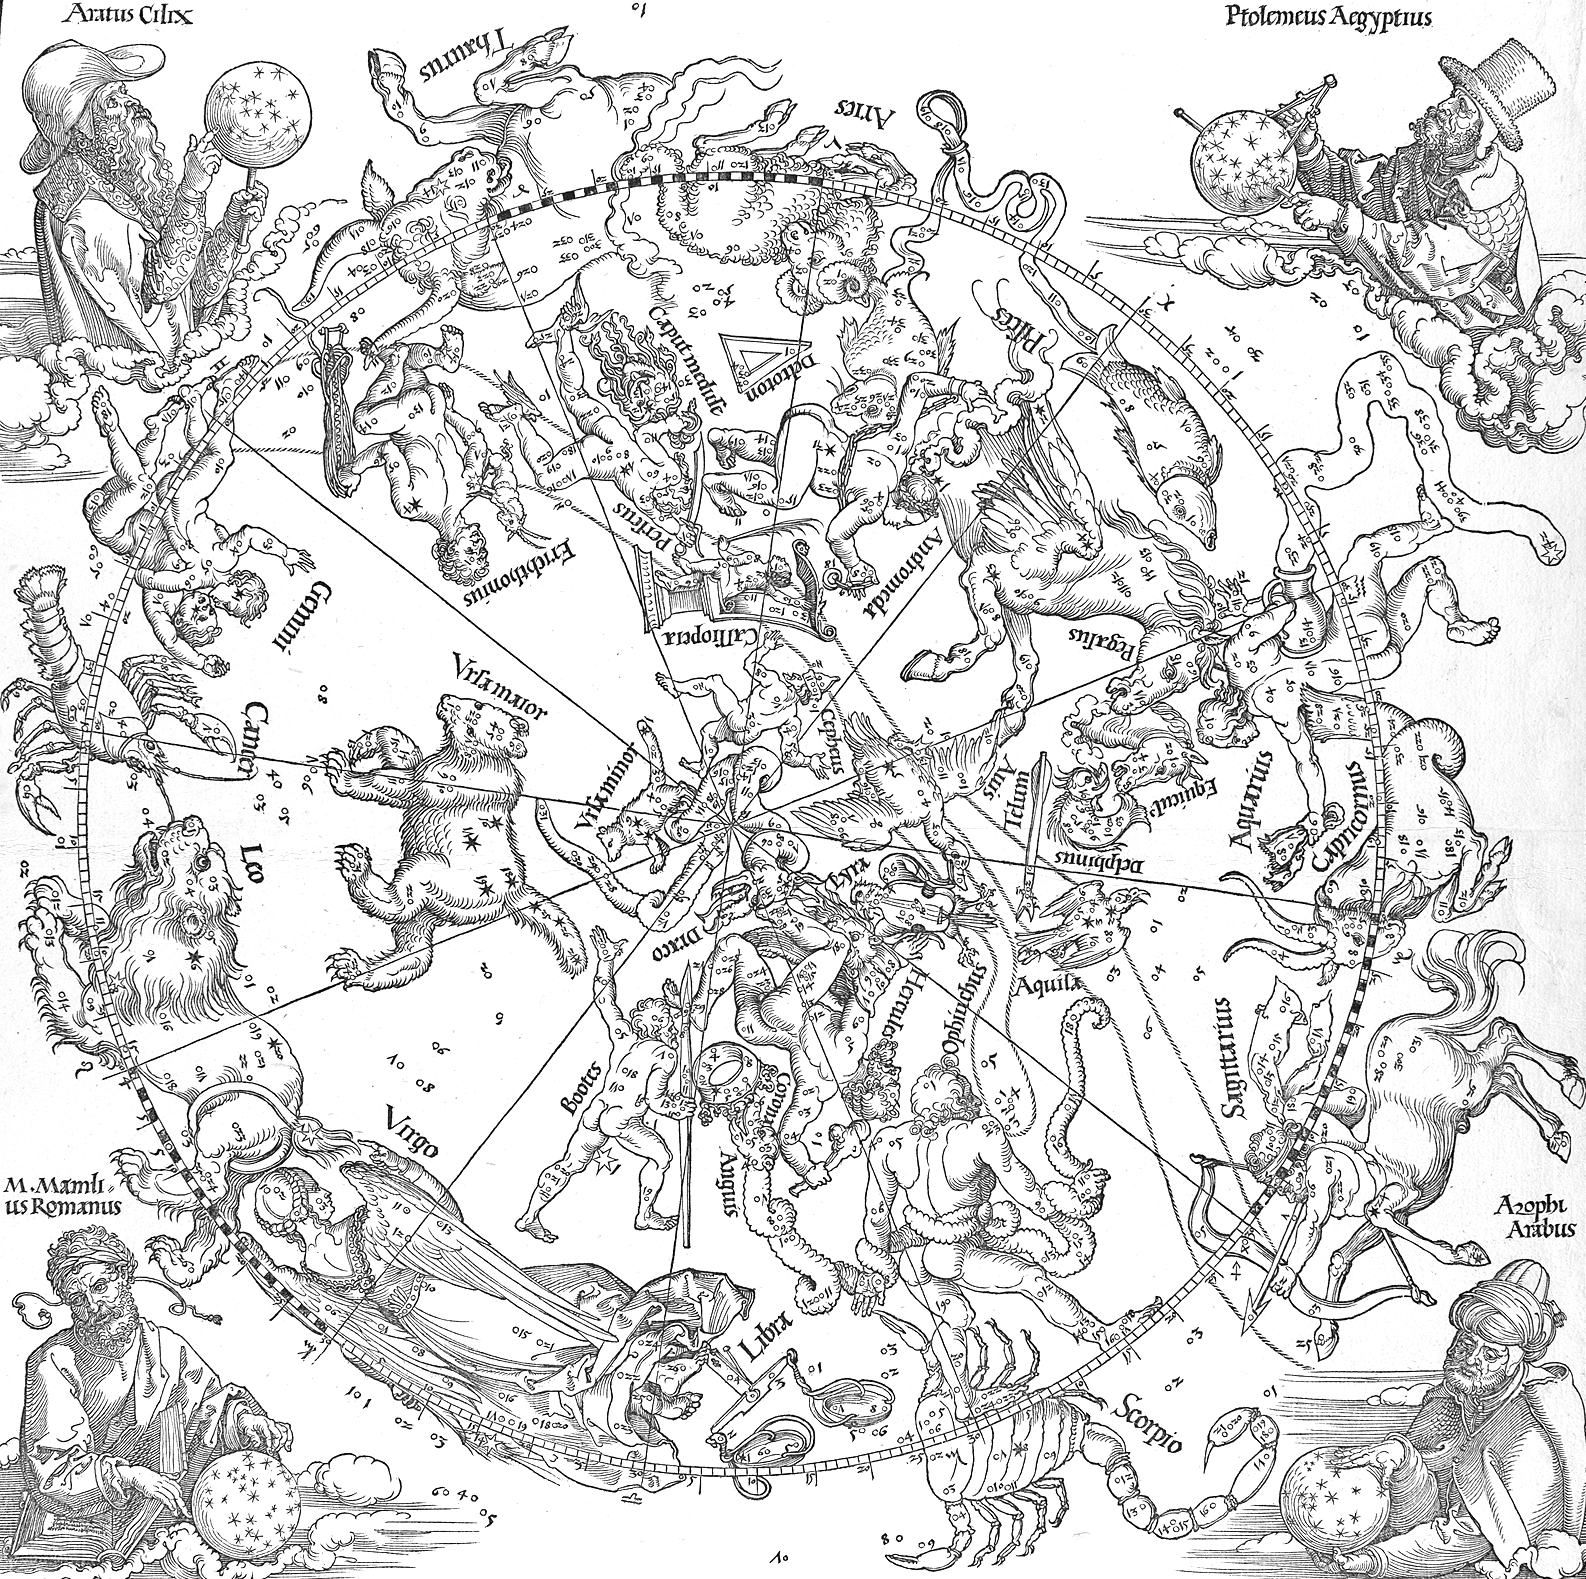
\includegraphics[width=0.82\linewidth]{images/durer_bw_level.png}
\end{center}
\vspace{0.1in}
\begin{center}
  
\includegraphics[width=0.28\linewidth]{images/sachiel_seal_plain.png}
\end{center}
\vfill
\begin{center}
  {\color{lightgrey}\rule{0.6\linewidth}{0.4pt}}\\[8pt]
  {\normalsize\itshape\color{darkgrey}
    The ceremony is an ani.mystic act of co-relating — you are attending to Sachiel, and Sachiel is attending to you.\\[6pt]
  }
\end{center}
\vfill
\begin{center}
  {\small\color{darkgrey} Prepared May 2026, v\docversion}\\[6pt]
  {\small\itshape\color{darkgrey} In remembrance of Gordon White (\dag 2026, age 27)}
\end{center}
\restoregeometry

\newpage

% ============================================================
% PREFACE
% ============================================================

\thispagestyle{empty}
\vspace*{0.4in}
{\normalsize

\noindent This booklet contains the rite for the Sachiel\,/\,Jupiter in Cancer
ceremony, with the hymns, prayers, and affirmations used in it.

\vspace{8pt}
\noindent \textbf{The purpose} is not petition for specific outcomes, but
conscious alignment with the Jupiter-in-Cancer current --- the energies of
home, nourishment, expansion, abundance, and meaningful travel that the cosmos
is already expressing during this window.

\vspace{12pt}
{\color{rubricsred}\itshape Timing}

\vspace{5pt}
\noindent\textbf{Full Moon in Sagittarius} \hfill {\footnotesize\color{darkgrey} May\,31, 2026 · 4:45am EDT}

\vspace{2pt}
{\footnotesize\color{darkgrey}\noindent%
\ps{⇧}~11Tau11 \enspace \ps{☉}~09Gem56 \enspace \ps{☾}~09Sag56 \enspace \ps{☿}~28Gem04 \enspace \ps{♀}~14Can39\\[1pt]
\ps{♂}~09Tau18 \enspace \ps{♃}~23Can57 \enspace \ps{♄}~12Ari12 \enspace \ps{♅}~02Gem02 \enspace \ps{♆}~04Ari03 \enspace \ps{♇}~05Aqu22\\[1pt]
\ps{★}~\ps{☉}/Aldebaran \enspace \ps{☾}/Antares \enspace \ps{♀}/Sirius \enspace \ps{♃}/Pollux \enspace \ps{☿}/Betelgeuse\\[1pt]
\ps{☾}\,\ps{△}\,\ps{♄}~applying \enspace \ps{☉}\,\ps{✶}\,\ps{♄}~applying \enspace \ps{☾}\,\ps{△}\,\ps{♆}~sep.%
}

\vspace{5pt}
\noindent\textbf{New Moon in Gemini} \hfill {\footnotesize\color{darkgrey} Jun\,14, 2026 · 10:54pm EDT}

\vspace{2pt}
{\footnotesize\color{darkgrey}\noindent%
\ps{⇧}~19Cap36 \enspace \ps{☉}~24Gem03 \enspace \ps{☾}~24Gem03 \enspace \ps{☿}~18Can32 \enspace \ps{♀}~01Leo57\\[1pt]
\ps{♂}~20Tau08 \enspace \ps{♃}~26Can51 \enspace \ps{♄}~13Ari19 \enspace \ps{♅}~02Gem52 \enspace \ps{♆}~04Ari17 \enspace \ps{♇}~05Aqu10%
}

\vspace{5pt}
\noindent\textbf{Jupiter (\ps{♃}) enters Leo} \hfill {\footnotesize\color{darkgrey} Jun\,30, 2026 · 1:13am EDT}

\vspace{2pt}
{\footnotesize\color{darkgrey}\noindent%
\ps{⇧}~02Ari23 \enspace \ps{☉}~08Can28 \enspace \ps{☾}~10Cap52 \enspace \ps{☿}~26Can15 \enspace \ps{♀}~19Leo19\\[1pt]
\ps{♂}~01Gem01 \enspace \ps{♃}~00Leo00 \enspace \ps{♄}~14Ari09 \enspace \ps{♅}~03Gem40 \enspace \ps{♆}~04Ari24 \enspace \ps{♇}~04Aqu53%
}

\vspace{5pt}
\noindent\rubric{Backup: any Thursday at sunrise while Jupiter is in Cancer.
Begin at actual sunrise --- not whenever you wake up.}

\vspace{12pt}
{\color{rubricsred}\itshape Materia}

\vspace{4pt}
\noindent 2 blue candles (Sachiel)
\quad 2 white candles (Moon)\\
Seal of Sachiel (blue, purple, or gold ink)\\
Offering bowl with blue offerings\\
Frankincense incense\\
Rosary, mala, or beads --- optional, for the affirmation

}

\mainmatter

% ============================================================
% SACHIEL & HIS LINEAGE
% ============================================================

\chapter*{Sachiel \& His Lineage}
\addcontentsline{toc}{chapter}{Sachiel \& His Lineage}
\thispagestyle{fancy}

{\normalsize

\noindent Sachiel is the angelic intelligence of Jupiter --- the apprehensible face of that
planetary current, the being you can actually meet. He governs Thursday, the fifth heaven,
and the qualities Jupiter has carried since antiquity: abundance, expansion, teaching,
generosity, meaningful travel, the wide road and the far horizon.

\vspace{6pt}
\noindent That a planet should have an angel is not a poetic conceit laid over astronomy from
the outside. It is how the heavens were understood for most of Western history. The biologist
Rupert Sheldrake puts the point plainly: the planets ``still bear the names of gods and
goddesses, like Mercury, Venus, and Jupiter, who in the Christian world were regarded as
angels,'' planetary intelligences ``with their different dispositions and relationships''
that ``affected life on earth.''\footnote{Rupert Sheldrake, in Matthew Fox and Rupert
Sheldrake, \textit{The Physics of Angels: Exploring the Realm Where Science and Spirit Meet}
(Rhinebeck, NY: Monkfish, 2014), from the introductory dialogue ``The Return of the Angels
and the New Cosmology.''} Jupiter and its angel are not two things. Sachiel is the face that
current turns toward us.

\vspace{6pt}
\noindent His lineage is old. The system of planetary angels --- one intelligence governing
each of the seven classical planets --- enters Western tradition through Jewish angelology,
and may trace further back through the Babylonian captivity to Sumerian sources, placing the
roots of this kind of spirit work somewhere around 20,000 years ago. The Barrett plate
reproduced at the back of this booklet shows Sachiel in his early modern ceremonial form:
fourth of seven, ruling Thursday, his seal a combination of the Jupiter glyph and the sign
of Cancer.

\vspace{6pt}
\noindent During Jupiter's transit through Cancer --- from mid-2025 through June 2026 ---
Sachiel carries a particular assignment. Cancer governs home, nourishment, embodiment, the
requirements of life. Jupiter in Cancer is the greater benefic in service of life itself.
Gordon White described Sachiel in this period as something like a diplomat on secondment:
same angel, new remit. The current he expresses is one of expansion rooted in belonging ---
not restless acquisition, but the abundance that comes from being genuinely, fully present
in your own life. There is warrant for this descent into the particular in the tradition
itself. Aquinas insisted that angelic government reaches all the way down into the
here-and-now: ``Administration and government and the causing of movement have to do with
particulars existing in the here and now.''\footnote{Thomas Aquinas, \textit{Summa
Theologiae} I, q. 57, a. 2, quoted in Fox and Sheldrake, \textit{The Physics of Angels},
ch. 2 (``St.\ Thomas Aquinas'').} An angel of abundance turned toward home and nourishment
is not a lesser angel. It is providence attending to the requirements of a life.

\vspace{6pt}
\noindent This ceremony stands inside a long tradition of Christian contemplative and
ceremonial practice --- longer and less interrupted than its modern reception might suggest.
The planetary angel system was not considered heterodox in medieval Christian thought.
Thomas Aquinas wrote seriously about angelic hierarchies and their governance of natural
phenomena. That God administered creation through angelic intermediaries was mainstream
theology --- in Aquinas's own words, ``the entire corporeal world is governed by God through
the angels,'' for ``the universe would not be complete without
angels.''\footnote{Thomas Aquinas, \textit{Summa Theologiae} I, q. 50, quoted in Fox and
Sheldrake, \textit{The Physics of Angels}, introduction and ch. 2.} Sachiel governing Jupiter
was simply how the cosmos was organized.

\vspace{6pt}
\noindent It is worth saying why this fell silent, because the silence is recent and not
inevitable. In the mechanical cosmology of the last few centuries there was no room for
angels --- there was, as Matthew Fox observes, no longer even much room for souls. But that
machine universe has itself been superseded by an evolving, living one, and Fox argues that
``the angels are returning because a living cosmology is
returning.''\footnote{Matthew Fox, in Fox and Sheldrake, \textit{The Physics of Angels},
introduction.} The point of this booklet is not nostalgia for a discarded picture. It is that
the picture was discarded prematurely, and the cosmos it described --- alive, populated by
intelligences, answerable to attention --- is the one a contemporary reader can once again
inhabit without embarrassment.

\vspace{6pt}
\noindent The Orphic hymns enter this lineage through Marsilio Ficino --- Renaissance
priest, philosopher, and translator --- who used them in what he called \textit{spiritus}
magic: drawing down planetary influences through music, scent, and invocation. He considered
this entirely compatible with Christian faith. His patron was Cosimo de' Medici. The hymns
in this booklet sit directly in that current.

\vspace{6pt}
\noindent The Seven Angels Prayer (Opening, Option~C) makes the Christian frame explicit.
Its structure --- Trinitarian, Christocentric, asking forgiveness before approaching the
angels --- follows standard cunning folk operating procedure: approach the angelic hierarchy
through Christ as mediator. Sachiel here is exactly what Aquinas would have recognized: a
ministering spirit operating within divine providence.

\vspace{6pt}
\noindent Florence Scovel Shinn, whose affirmation closes the ceremony, was a Christian
metaphysician in the New Thought tradition --- deeply scriptural, treating affirmation not
as wishful thinking but as declaration of what divine will is already doing. The words are
simple; the theology underneath them is precise.

\vspace{6pt}
\noindent The thread connecting all of these is Christian Neoplatonism --- running from
Pseudo-Dionysius the Areopagite through Ficino and Pico della Mirandola --- which held that
the cosmos is a hierarchy of intelligences emanating from God, and that the contemplative
practitioner could consciously align with that hierarchy through prayer, beauty, attention,
and right timing. Sachiel is not a rival to God in this understanding. He is an expression
of divine generosity made relatable. In Dionysius's terms, to take one's place consciously
within that order is to become ``a fellow-worker with God,'' showing forth the divine
activity ``as far as possible in himself.''\footnote{Pseudo-Dionysius the Areopagite,
\textit{The Celestial Hierarchies}, quoted in Fox and Sheldrake, \textit{The Physics of
Angels}, ch. 1 (``Dionysius the Areopagite''). The phrase echoes 1 Corinthians 3:9.} That
older language of the co-worker is the root of what this ceremony calls co-relating.

\vspace{6pt}
\noindent This is not a syncretism assembled from parts. It is a single tradition, viewed
from several windows.

\vspace{10pt}
\noindent The ceremony that follows is an invitation to align consciously with that current.
Not to petition Sachiel for outcomes, but to meet him --- and to let him meet you. As Fox
glosses Aquinas: the angels ``always announce the divine silence, the silence that precedes
our own inspiration, our own words, the silence that meditation and contemplation
bring.''\footnote{Matthew Fox, in Fox and Sheldrake, \textit{The Physics of Angels}, ch. 2,
glossing Aquinas. Compare the Orphic Hymn to Sachiel below: ``the golden hush that precedes
discovery.''} That silence is what you are sitting in when you sit in presence. The noticing
is the whole of it.

}

% ============================================================
% THE CEREMONY
% ============================================================

\chapter*{The Ceremony}
\addcontentsline{toc}{chapter}{The Ceremony}
\thispagestyle{fancy}

\rubric{Set up your materia before beginning. Light the incense as you open.}

\ornsep

% ============================================================
% I. OPENING
% ============================================================

\section*{I. Opening}

\vspace{6pt}
\begin{center}
  {\normalsize\itshape\color{darkgrey}
    ``If this is the first time you ever do a ceremony,\\
    you're not going to mess this up.\\
    You're basically dealing with God, the moon,\\
    and the angel of Jupiter.\\
    Nothing's going to go sideways here.''
  }\\[6pt]
  {\footnotesize\color{darkgrey} ---~Gordon White}
\end{center}

\ornsep

\subsection*{Choose one of the forms below}

\rubric{Begin by sanctifying the space. The specific method matters less than
the intention. Three forms are given; use the one most natural to you.}

\vspace{8pt}

\subsection*{Option A \hspace{0.5em} Divine Light Invocation}

\prayerblock{%
  I call upon the Divine Light ---\\
  Source of all that is good, true,\\
  and beautiful.\\[8pt]
  Fill this place.\\
  Fill this body.\\
  Fill this hour.\\[8pt]
  Let only that which serves\\
  the highest good be present here.\\[8pt]
  May this space be consecrated.\\
  May this ceremony be sealed in light. Amen.
}

\ornsep

\subsection*{Option B \hspace{0.5em} The Lord's Prayer}

\prayerblock{%
  Our Father, who art in heaven, hallowed be thy name.
  Thy kingdom come. Thy will be done, on earth as it is in heaven.
  Give us this day our daily bread. And forgive us our trespasses, as we forgive those who trespass against us.
  And lead us not into temptation: but deliver us from evil.
  Amen.
}

\ornsep

\newpage
\subsection*{Option C \hspace{0.5em} Seven Angels Prayer\protect\srcmark}
\srcnote{English cunning folk\,/\,ceremonial magic manuscript tradition,
likely 17th--18th century. Source unidentified; possibly related to the
\textit{Book of Oberon} (British Library MS Harley 3981) or the Heptameron
tradition as adapted by English cunning men. The seven angels follow the
Chaldean planetary order: Cassiel (Saturn), Sachiel (Jupiter), Samael (Mars),
Michael (Sun), Anael (Venus), Raphael (Mercury), Gabriel (Moon).}

\prayerblock{%
  Oh infinite, wise, holy, blessed,\\
  glorious, pure, good, omnipotent\\
  Father, Son and Holy Ghost,\\
  one true god of gods,\\
  king of kings, lord of lords,\\
  creator of all the universal world,\\
  the holy, holy, holy,\\
  high, good and merciful Sabaoth,\\
  the omnipotent of all powers\\
  in whom all creatures live, move and be,\\
  and do obey to thee,\\
  which hast created thine angels in wonderful order\\
  and made them thy ministering spirits\\
  for all believers and heirs of salvation\\
  to the glory of thy great and holy name.\\[8pt]
  
  I, thine unworthy servant, do humbly implore\\
  thy holy, divine, glorious \\
  good and merciful majesty,\\
  through thine infinite goodness \\
  and love and mercy\\
  and eternal love of Jesus Christ,\\
  our mediator and messiah,\\
  that you will vouchsafe \\
  to forgive my manifold sins\\
  and to purify my mind, soul, spirit and body\\
  with thy Holy Spirit,\\
  and fortify me with true faith, hope and charity,\\
  and grant me virtue and power\\
  that these, thy holy angels;\\
  Cassiel, Sachiel, Samael, Michael,\\
  Anael, Raphael, and Gabriel;\\
  with their ministering angels and spirits\\
  being called or required\\
  in the name of God the Father, \\
  Son and Holy Ghost,\\
  may through thy mercy in Jesus Christ,\\
  willingly and readily teach, instruct,\\
  show and visibly represent,\\
  openly and plainly in my native tongue,\\
  make me perfectly to understand clearly\\
  all my honest and lawful desires,\\
  questions or demands.\\[8pt]
  And in all my necessities,\\
  with perfect understanding and memory,\\
  help and confirm me with thy power\\
  and strength and wisdom and might\\
  against all assaults of mine enemies,\\
  spiritual and bodily.\\
  To thy glory, good of thy people\\
  and comfort of me, thine unworthy servant,\\
  through thine eternal love and mercy\\
  in Jesus Christ, our lord and saviour,\\
  so be it done.\\[8pt]
  And in the name of God the Father, Son and Holy Ghost,\\
  to whom be ascribed all honour, glory, power,\\
  might, majesty and dominion without end.\\[8pt]
  Amen.
}

\ornsep

\subsection*{Option D \hspace{0.5em} Your own opening}

\rubric{A shamanic opening, a calling-in of allies and guides, or any practice
already belonging to your personal tradition. Spend at least a minute here.
The point is sanctifying the space, not the specific form.}

\ornsep

% ============================================================
% II. ORPHIC HYMN TO THE MOON
% ============================================================

\section*{II. Orphic Hymn to the Moon\protect\srcmark}
\srcnote{Trans.\ Apostolos N. Athanassakis and Benjamin M. Wolkow,
\textit{The Orphic Hymns} (Johns Hopkins University Press, 2013), Hymn~9.}

\subsection*{To Selene}

\rubric{The text indicates incense: aromatic herbs; we're using frankincense.}

\vspace{6pt}
\prayerblock{%
  Hear me, O divine queen,\\
  O light-bringing and splendid Selene,\\
  O bull-horned Moon,\\
  crossing the air as you race with night.\\[8pt]
  Nocturnal, torch-bearing,\\
  maiden of beautiful stars, O Moon,\\
  waxing and waning,\\
  feminine and masculine,\\
  luminous, lover of horses,\\
  mother of time, bearer of fruit,\\
  amber-colored, moody,\\
  shining in the night,\\
  all-seeing and vigilant,\\
  surrounded by beautiful stars,\\
  you delight in the quiet\\
  and in the richness of the night,\\
  you grant fulfillment and favor\\
  as, like a jewel, you shine in the night.\\[8pt]
  Long-cloaked marshal of the stars,\\
  wise maiden whose motion is circular,\\
  come, O blessed and gentle lady,\\
  lady of the stars, through your own light\\
  shine and save, O maiden,\\
  your new initiates.
}

\ornsep

% ============================================================
% III. ORPHIC HYMN TO SACHIEL
% ============================================================

\section*{III. Orphic Hymn to Sachiel\protect\srcmark}
\srcnote{Gordon White, \textit{Rune Soup}, ``Full Moon In Sagittarius Ritual: Bring Me That Horizon'' (Jun.\ 2025).
\texttt{https://www.youtube.com/watch?v=0yV7du5lz14}}

\prayerblock{%
  O Sachiel, Radiant One,\\
  Keeper of the Benevolent Flame,\\
  You who wear the mantle\\
  of the sky's wide order,\\
  Whose breath is the spring wind\\
  that awakens all things ---\\
  Come now to this place,\\
  Where the moon is full\\
  and the heart is open.\\[8pt]
  Bless\'ed are you,\\
  who gives freely and asks only readiness.\\
  You stir the wise to speak,\\
  the wanderer to walk,\\
  You plant visions in the minds of those\\
  Who dare to ask for more than safety.\\[8pt]
  Let your light fall upon this threshold.\\
  Not as blinding glory,\\
  but as the golden hush\\
  that precedes discovery.\\
  Let your signs be many,\\
  and your silence be brief.\\[8pt]
  Bring teachers with eyes like lanterns.\\
  Bring companions whose laughter rings true.\\
  Bring trials that shape but do not break.\\
  Bring roads that are longer\\
  than maps allow.\\[8pt]
  O Prince of Peaceful Power,\\
  Crowned in amethyst, clothed in thunder,\\
  Pour your blessings\\
  into this willing vessel.\\
  Make of me a pilgrim\\
  who finds what he seeks ---\\
  And more, always more.\\[8pt]
  So be it,\\
  As the stars are many\\
  And the path is long.
}

\ornsep

% ============================================================
% IV. A HYMN TO SACHIEL
% ============================================================

\section*{IV. A Hymn to Sachiel\protect\srcmark}
\srcnote{Composed by Claude Sonnet 4.6 and Icculus, 2026.}

\prayerblock{%
  O Sachiel, great keeper of the generous current,\\
  You who move through the mansions of heaven\\
  Like a tide that lifts all vessels ---\\
  I have lit this flame so you might find me.\\[8pt]
  You are the wide road and the open gate,\\
  The teacher who arrives before you are expected,\\
  The abundance that does not announce itself\\
  Until it is already in your hands.\\[8pt]
  I come to you not with a list of wants\\
  But with attention --- which is all I have,\\
  Which is, they say, everything.\\
  Here it is. It is yours.\\[8pt]
  Meet me here, across this threshold,\\
  In the blue hour, in the gold light,\\
  In the amethyst space between asking and receiving.\\
  Let us come to know each other.\\[8pt]
  I align myself with your mission:\\
  Life, embodiment, the fullness of things,\\
  The heart that has enough and knows it,\\
  The road that is longer than the map allows.\\[8pt]
  Move through me as water moves through a willing land.\\
  I am ready to be the fulfillment of this current.\\
  New fields open. Unexpected doors fly open.\\
  Unexpected channels are free.\\[8pt]
  So be it.
}

\ornsep

% ============================================================
% V. OFFERINGS
% ============================================================

\newpage
\section*{V. Offerings}

\rubric{Place your blue offerings in the bowl.
Light the frankincense if not already burning.
Light the candles.}

\vspace{8pt}
\rubric{Spend a moment in the light and the scent before moving on.
There is no formula here --- just presence and intention.}

\ornsep

% ============================================================
% V. SITTING IN PRESENCE
% ============================================================

\section*{VI. Sitting in Presence}

\begin{center}
  {\normalsize\itshape\color{darkgrey}
    ``Sit there smelling the frankincense\\
    and just notice.''
  }\\[6pt]
  {\footnotesize\color{darkgrey} ---~Gordon White}
\end{center}

\vspace{4pt}
\rubric{Spend time quietly in the space --- candles, incense, nighttime.
Do not rush this. You may receive something;
you may simply absorb the atmosphere. Both are fine.}

\vspace{8pt}
\rubric{The witchcraft writer Lee Morgan suggests that the sight ---
the traditional name for spiritual perception --- could almost be called
\textit{the noticing}. It is not a rare gift you either have or lack.
It is sustained, honest attention to what is actually present.
That is the whole practice.\protect\srcmark}
\srcnote{Gordon White, \textit{Rune Soup}, ``Full Moon In Sagittarius Ritual: Bring Me That Horizon''
(Jun.\ 2025). \texttt{https://www.youtube.com/watch?v=0yV7du5lz14}}

\vspace{8pt}
\prayerblock{%
  \textit{What is present here?}\\[4pt]
  \textit{What do I notice?}
}

\ornsep

% ============================================================
% VI. AFFIRMATION
% ============================================================
\newpage
\section*{VII. Affirmation\protect\srcmark}
\srcnote{Florence Scovel Shinn (1871--1940), \textit{The Game of Life and
How to Play It} (1925).}

\subsection*{Florence Scovel Shinn}

\rubric{Use beads if you have them. Repeat multiple times; Let it settle into the body.}

\vspace{8pt}
\prayerblock{%
  \textit{``New fields of divine activity now open for me.\\
  Unexpected doors fly open.\\
  Unexpected channels are free.''}
}

\ornsep

% ============================================================
% VII. CLOSING
% ============================================================

\section*{VIII. Closing}

\rubric{Thank Sachiel --- Gordon frames this like saying goodbye to a guest.
A license to depart. Brief is sufficient; sincerity matters more than length.}

\vspace{8pt}
\prayerblock{%
  Sachiel, Radiant One ---\\
  I give thanks for your presence here.\\
  Go in peace, and return when called.
}

\vspace{10pt}
\rubric{Blow out the candles. The ceremony is complete.}

\ornsep



% ============================================================
% INTERLEAF IMAGE
% ============================================================

\clearpage
\thispagestyle{empty}
\vspace*{\fill}
\begin{center}
  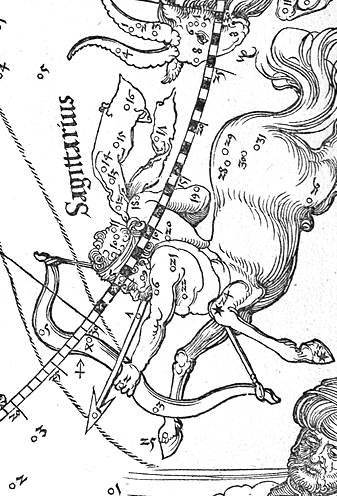
\includegraphics[width=0.5\linewidth]{images/durer_celestial_north_sag_level.png}
\end{center}
\vspace*{\fill}
\clearpage

% ============================================================
% ONGOING PRACTICE
% ============================================================

\chapter*{Ongoing Practice}
\addcontentsline{toc}{chapter}{Ongoing Practice}
\thispagestyle{fancy}

\rubric{The ceremony is a beginning, not a conclusion.}

\vspace{10pt}
\prayerblock{%
  Add Sachiel's seal to your altar if you have one.
  Light a candle on Thursday mornings occasionally.
  Practice ongoing noticing --- watch for synchronicities
  along Jupiter-in-Cancer themes:\\
  home, nourishment, expansion, abundance,\\
  meaningful travel.
}

\ornsep

\vspace{6pt}
{\normalsize\itshape\color{darkgrey}
\noindent The goal is not to petition for specific things,
but to signal conscious alignment with the Jupiter in Cancer current ---
to become an intentional co-expresser
of what the cosmos is already doing.
}

\vspace{8pt}
\attribution{Gordon White, Rune Soup (Jun.\ 2025)}

% ============================================================
% IMAGE CREDITS
% ============================================================

\clearpage
\newgeometry{top=0.5in, bottom=0.5in, inner=0.65in, outer=0.55in}
\thispagestyle{empty}

{\footnotesize\color{darkgrey}
\sloppy

\noindent\textbf{Books}

\vspace{6pt}
\noindent Matthew Fox and Rupert Sheldrake. \textit{The Physics of Angels: Exploring the
Realm Where Science and Spirit Meet}. Rhinebeck, NY: Monkfish, 2014. Originally published
1996. A dialogue between a theologian and a biologist, working through Pseudo-Dionysius,
Aquinas, and Hildegard of Bingen on the nature and function of angels. The source for the
Aquinas and Dionysius quotations in the lineage notes.

\vspace{6pt}
\noindent Gordon White. \textit{Ani.Mystic}. Scarlet Imprint, 2023. A sequel to
\textit{Star.Ships}, and explicitly a magician's book: an exploration of animism --- ``the
belief that the world is made up of persons, only some of whom are humans'' --- taken to its
farthest epistemological hinterlands. Drawing on Indigenous knowledge, field encounters
across Papua New Guinea, Aboriginal Australia, and Peru, and the Western magical tradition,
it makes the case for a cosmos populated by real intelligences, answerable to attention.

\vspace{10pt}
\noindent\textbf{Videos}

\vspace{6pt}
\noindent Gordon White. ``Full Moon In Sagittarius Ritual: Bring Me That Horizon.''
\textit{Rune Soup}, Jun.\ 7, 2025.\\
\texttt{https://www.youtube.com/watch?v=0yV7du5lz14}\\
The source video for this booklet: the ceremony structure, the Orphic Hymn
to Sachiel, the Florence Scovel Shinn affirmation, the Lee Morgan framing
of the sight as the noticing, and the broader context of Jupiter in Cancer
as a current of home, nourishment, expansion, and meaningful travel.

\vspace{10pt}
\noindent\textbf{Images}

\vspace{8pt}
\noindent Albrecht D\"urer (1471--1528). \textit{The Celestial Map --- Northern
Hemisphere}, 1515. Woodcut; sheet: 61.3 $\times$ 45.6\,cm.
The Metropolitan Museum of Art, Harris Brisbane Dick Fund, 1951.
Public domain (CC0).

\vspace{6pt}
\noindent Francis Barrett (1774--\textit{fl.}\,1801). \textit{The Magus, or
Celestial Intelligencer}, London: Lackington, Allen and Co., 1801. Plate:
``A Table shewing the names of the Angels governing the 7 days of the week,
with their Sigils, Planets, Signs \&c.'' Engraving with hand colour. Public domain.

}

\vspace{10pt}
\begin{center}
  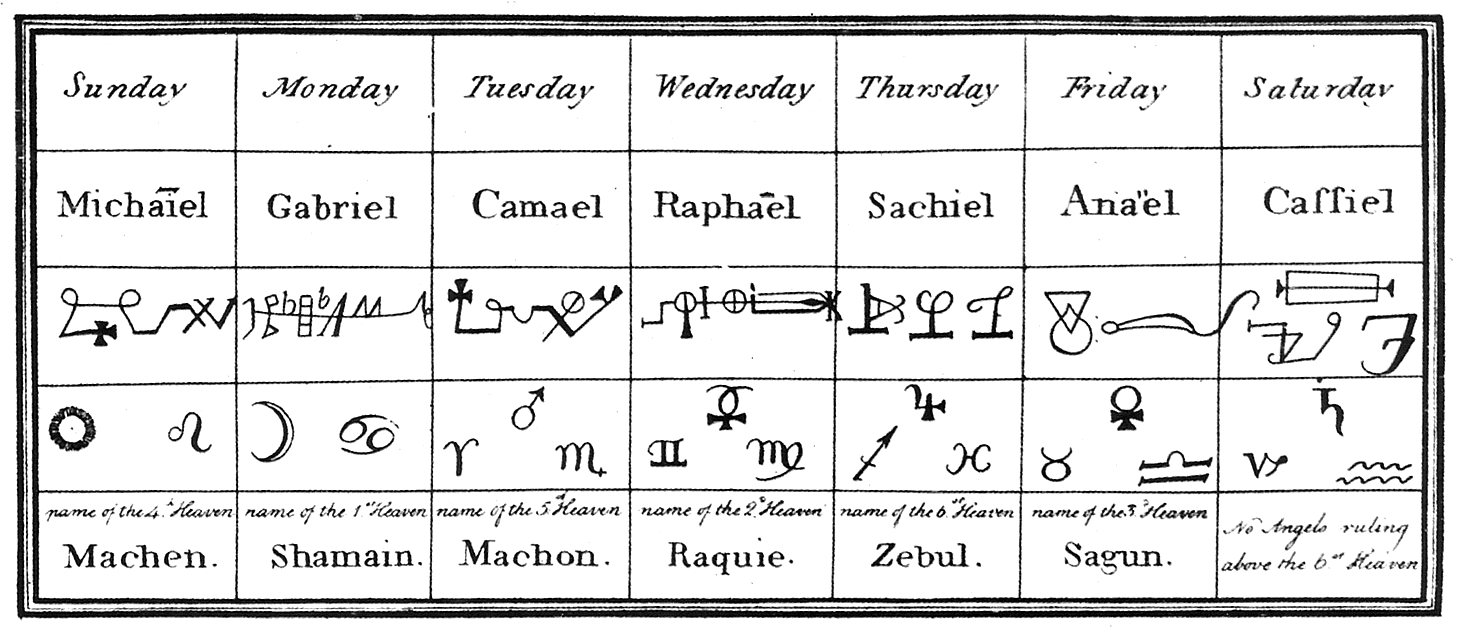
\includegraphics[width=0.75\linewidth]{images/barret_seals_clip_level.png}
\end{center}
\vspace{4pt}
{\footnotesize\itshape\color{darkgrey}\centering
  The seals of the seven days from Barrett's plate. Thursday (Sachiel) is the fourth seal.
\par}

\vspace{6pt}
{\footnotesize\color{darkgrey}
\begin{center}
  {\small\color{deepgold} Temple of the Exalted Lantern} \quad
  \texttt{icculus@templeofexla.com} \\
  {\itshape with gratitude to the RSPM}\\[4pt]
  \textcopyright\ 2026 Temple of the Exalted Lantern \textbullet\
  CC BY-NC-SA 4.0 \textbullet\
  \texttt{creativecommons.org/licenses/by-nc-sa/4.0}
\end{center}
}

\restoregeometry

\end{document}
